\chapter{Design and Implementation}
This chapter will detail the design and implementation of the PEEPS framework. It begins by discussing the various design proposals which developers should take into consideration when developing an app of this type, and then using these proposals it will justify the final design of the app and server components. Subsequently, this chapter will discuss the system level view of the project before detailing the finer aspects of each subsystem within the PEEPS framework.

\section{Conceptual Design}
Due to the malleable and open nature of software engineering, it is useful to take aspects of each system and interrogate how it is best to approach them. This chapter will detail that process by looking at the options available for each major system concept and provide insight into how different approaches can take the application in different directions. This chapter will also justify why particular options were chosen over the alternatives.  

\subsection{Concept Design Proposals}
\label{sec:design_proposals}

\subsubsection{A. Smartphone Application Operating System}

For mobile application development there are always two operating systems that need to be considered: Google's Android and Apple's iOS. Combined, these two mobile operating systems make up 99.42\% of the global smartphone market \cite{StatCounter} and applications for each of these operating systems are unique both in their design and development strategy. The choice of which of these OS's to target determines the application's audience, development software and documentation resources. As a result, this decision is best made early in the development lifecycle. Each operating system also has its own development language and first-party development applications that allow for a seamless development strategy. 

Proposals:

\begin{enumerate}
    \item \textbf{Android, programmed using Java:} Android devices make up over 74\% of global mobile smartphones, making android development the most beneficial in terms of potential reach \cite{StatCounter}. Google released the development environment Android Studio in 2014, which provides a variety of application frameworks for jumpstarting development. The official language for Android app development is Java which has a large backlog of libraries and other resources from its 20+ years of existence, making it ideal for both new developers and experienced veterans. 
    \begin{figure}[H]
        \centering
        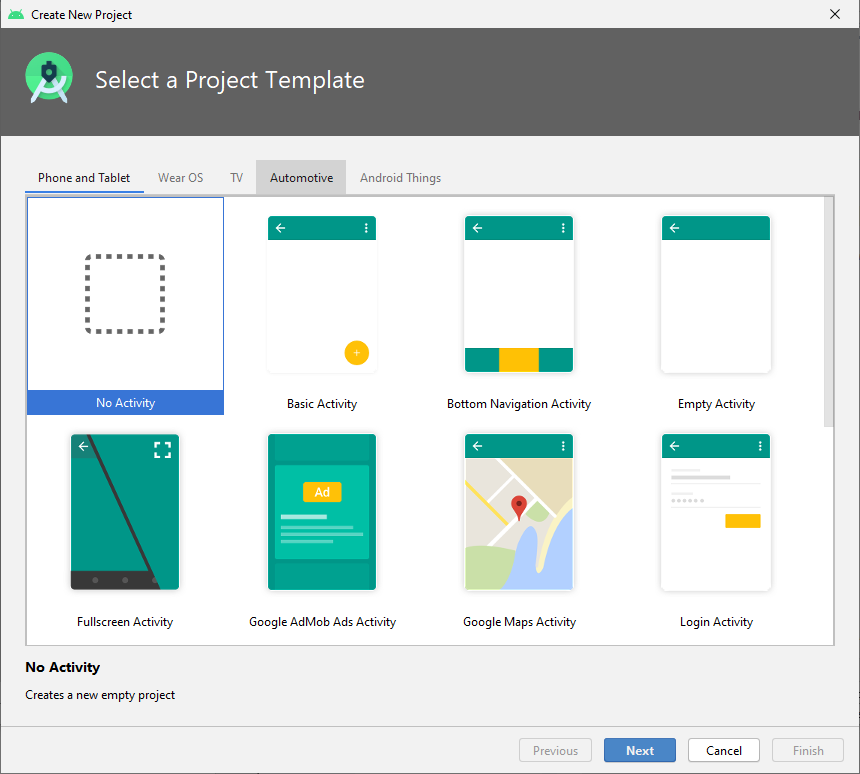
\includegraphics[width = .7\linewidth]{figures/AndroidStudioTemplates.PNG}
        \caption{Android Studio's activity templates used to jumpstart development.}
    \end{figure}
    \item \textbf{iOS, programmed using Swift:} While iOS devices are less common globally, their large market share in the US always make them an option worth considering. Unfortunately for the scope of this project, it is much harder to find enough apple devices for mass testing due to android smartphone prevalence. Swift is Apple's first-party programming language unveiled in 2014, making it much younger than Android's alternative. Due to its youth, the developers of Swift have drawn techniques from established programming languages to create a modern language that is learner-friendly and robust. However, this comes with the downside of a lack of available documentation and troubleshooting resources. Swift's support from Apple does means that it is tailored to iOS application development, making it a tempting choice for new developers who want a programming language tailored to them. 
    \item \textbf{Android and iOS, programmed using Flutter \& Dart:} Flutter is Google's foray into programming language development. Its purpose is to bridge the gap between Android and iOS development, providing an engine that can compile a codebase for both platforms. Flutter uses Dart, an object orientated programming language also developed by Google, to write programs compatible with both platforms. Much like Swift, Dart is relatively new, making its documentation and troubleshooting resources more limited than alternatives. Fortunately for Flutter, its dual operating system approach makes it extremely valuable when one's goal is to develop for both platforms. Unfortunately, because Flutter's objective is to be used to create for both platforms, it still relies on Java and Swift for some background service functionality.
\end{enumerate}

\subsubsection{B. Database Type}

While the choice of database will have some impact on how data will be stored from the smartphone application, most databases are very similar in their makeup, and choosing one is more of a preference than it is a significant design decision. What will change between databases is the various extensions that can be used, the databases' available datatypes, and their method of interacting with web interfaces.

Proposals:

\begin{enumerate}
    \item \textbf{MySQL:} MySQL is one of the most popular databases for a variety of reasons: it is free, has extensive functionality and has plenty of user interfaces that can be chosen from. By using the free version, you will be missing out on some of the more advanced features, but this is offset by the sheer robustness of MySQLs database implementation.
    \item \textbf{SQLite:} SQLite is a versatile database that is great for quickly creating databases that are reliable, portable, and lightweight. However, it has disadvantages of not being built for high levels of HTTP requests and of having a database size limit. These factors make it not as desirable as alternatives for applications that need high scalability.
    \item \textbf{PostgreSQL:} PostgreSQL is a database implementation that has plenty of advantages over its competition. It allows for both structured and unstructured data, is highly scalable, supports JSON, and has plenty of available extensions. A relevant extension to this project is PostGIS which allows PostgreSQL to handle complex geometric data.
\end{enumerate}

\subsubsection{C: Web Application Software}

To interact with a database run from a server over HTTP, you will need to implement some form of web interface. This can be done by developing software designed to interact with incoming HTTP requests. This type of web development is typically done using the PHP language, but Python has made itself a compelling alternative with its functionality extending beyond just web applications. For purely web development, both can perform the job, but the choice between them may rest on how much you value Python's large suite of unique libraries over the more established PHP landscape.

Proposals:

\begin{enumerate}
    \item \textbf{Python:} It is assumed amongst software engineers that for any project, there is usually a python library or framework that could help you accomplish it. Web development, in this case, is no exception. With the introduction of the Django web framework, Python has made itself a strong alternative to the more established PHP. The sheer versatility of this programming language means that when using Django, you have access to far more functionality than just web development. Additionally, Python has a simple, but elegant syntax that can be easily understood by newer developers. 
    \item \textbf{PHP:} PHP is a language used strictly for web development. Its popularity in the web application space means that it's the language of choice for large web-based companies like Facebook, Wikipedia and Tumblr \cite{ThePHPGroup}. Its `C'-style syntax means that it is easy to pick up for developers new to the language, and its persistence since its inception means that there are plenty of resources available to you as you develop your application. While Python is more popular than PHP for general use applications, PHP is still far more popular when it comes to web applications \cite{ThePHPGroup}. The choice between them may come down to whether you plan to make use of Python's large number of applications or stick to purely web development.
\end{enumerate}

\subsection{Final Design Decision}

This section details the design choices made between the options presented in Section \ref{sec:design_proposals}. Note that for any combination of mobile OS, database type and web application software, insights gained from this project will still be relevant. Each proposal option is one that could be justified, and which is most appropriate for your own project will be dependent on your developmental goals and perspective. 

\textbf{A.} The Android mobile operating system was chosen as the designated development platform for this project. Android was chosen primarily for its greater reach globally, making the results of the project more relevant to the average developer. Additionally, Java has far more available resources in terms of forum interactions and tutorials, speeding up the development process for complex systems like background processes and location-tracking activities. This decision is the one that has the least transferable results between related population density mobile apps, as it only takes into consideration the Android use-case and ignores the differences in results that will be caused by developing for iOS instead. The operating systems are similar enough where the insights gained will still be relevant, but iOS developers should be aware that not all results may map exactly to Apple's ecosystem.

\textbf{B.} PostgreSQL was chosen as the preferred database for this project. The PostGIS extender for PostgreSQL allows for seamless geographical object interaction which is perfect for this project's use-case. This makes PostgreSQL the clear choice over its alternatives. If developers were to use other database types, locational data could instead be stored as vector types or one could split the latitude and longitude values into individual float values. Developers using different databases should be aware that much of the interaction between the web application and the database is easily transferable between databases, and the difference in performance testing should be minimal.

\textbf{C.} The web application language chosen for this project is PHP as the scope of the server software has no need for the extended capabilities of the Python language. Since PHP is more commonly used, the development insights and codebase should be more applicable for developers wishing to use the PEEPS application framework. Should developers want to expand the capabilities of their web application, Python is the recommended solution.

With the main proposals for the PEEPS application framework finalised, it is possible to start designing the subsystems that will act as independent modules capable of being incorporated into any population tracking application. These subsystems will still be relevant for developers choosing alternative programming methods, as the discussion will still be at a high level of abstraction. 

\section{The PEEPS Application Structure}
With these design decisions justified, it is now possible to explain in depth the system level analysis for this project. This section will detail the system level design decisions taken when developing the application to be run on mobile devices.
\subsection{System Level Overview}

\begin{figure}[ht]
\centering
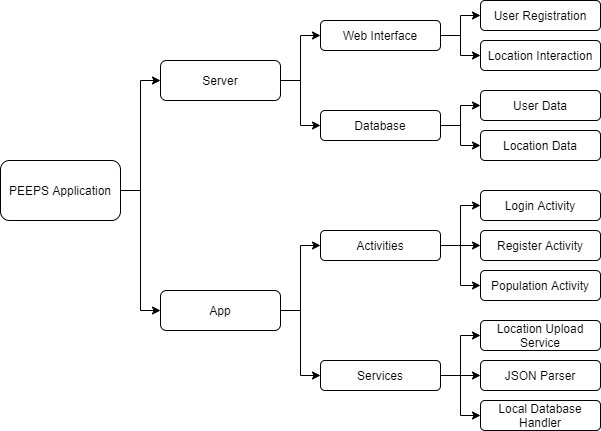
\includegraphics[width=0.8\textwidth]{figures/SystemHighLevel.png}
\caption{High level overview of the main application systems and their components.}
\label{fig:system_high_level}
\end{figure}

The design of the PEEPS framework is split into two independent systems: the smartphone application and the server. Each of these systems is independent in the sense that one could be swapped out with little change in the operation of the other system. The application could upload to a different server type or the server could receive data from a different application and the fidelity of the overall framework will remain operational. The inter-system interactions will be summarised in Section \ref{sec:Inter-System Interaction Summary} and will be discussed in more detail in each subsystem's section.

\subsection{Inter-System Interaction Summary}
\label{sec:Inter-System Interaction Summary}
Since the server system acts as the `hub' for all the stored user and locational data, it will only interact with the mobile application when information is requested by the application. This will happen when two conditions are met: either the application wants to retrieve or store user login data, or the application wants to retrieve or store geographical data. When this is not happening, the server will remain dormant, while still being accessible by backend managers who wish to interact manually with the data. Likewise, the smartphone application can still run without a connection to the server, although its functionality will be severely reduced. 

\subsection{Data Anonymity}
Because of the sensitive nature of population tracking and the possibility of abuse, all data displayed to the user by the PEEPS system is predicted from past data and is completely anonymous. Should live population data be displayed, malicious users could abuse the system to perform illegal acts such as theft. Therefore, the PEEPS system uses anonymous prediction mechanisms to provide useful insight into probable location-populations without compromising individuals' or businesses' privacy and safety. 

\section{App Design and Development}
\subsection{System Description}
The Peeps smartphone application can be split into three main subsystems: The login subsystem, the register subsystem, and the population-density subsystem. The fundamental aspect which separates these subsystems is their unique Java activity which handles the application's UI and its interaction with the user.  The login and register subsystems administer the user's identification and registration within the PEEPS app. They allow the user to create an account and access the app's main functionality by logging into the app using that account. When a user has successfully logged in, it will be able to interact with the application's population-density subsystem. This subsystem provides the bulk of the application's functionality, which is split into the `saved location' and `mapmode' fragments. These are discussed in more detail in Section \ref{sec:Subsystem Analysis}.

\subsection{Java Class Structure}

\begin{figure}[ht]
    \centering
    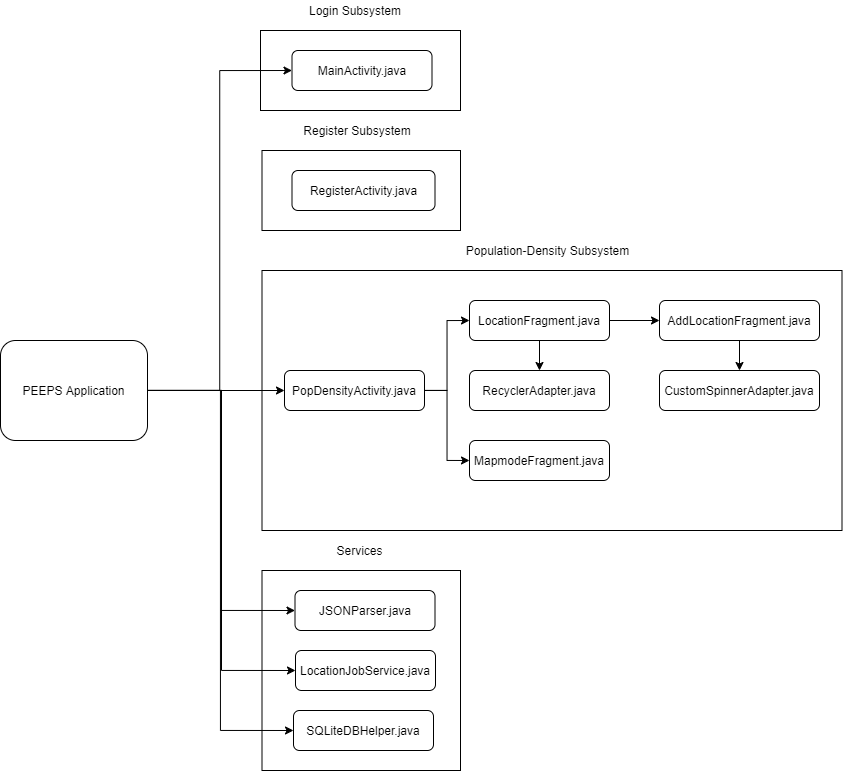
\includegraphics[width=0.8\textwidth]{figures/ClassDiagram.png}
    \caption{Java class hierarchy for the PEEPS App.}
    \label{fig:class_diagram}
\end{figure}

Android applications are typically built using a combination of Java class files and xml resource files. The classes act as the method by which the app can receive, interpret, and manipulate information where the xml files are templates which are used by the app to display application artifacts to the user. Because of the modular nature of programming, it is possible to fracture the structure of the application into various types of components. The main components which the application makes use of are as follows:

\textbf{Activities}

Activities are the highest-level class in the application hierarchy. These classes manipulate the UI and handle all the interaction performed between the user and the app. For example, when a user attempts to access a new screen on the app, the activity will have to handle this transition. In the PEEPS app, each activity is its own subsystem which provides some unique functionality to the user. The three activities in this application are the login activity, register activity and population-density activity.

\textbf{Layouts}

Layouts are the blueprints used to create the application GUI. These are coded in xml and are interacted with using their Java class. These layouts can describe either entire activity UIs or individual components of an activity's interface.

\textbf{Fragments}

Fragments are GUI elements and Java classes which are used by activities to display different UI's without transitioning to a new activity. In this application, Fragments are used by the population-density activity to perform different interactions with the user, each with a unique GUI.

\textbf{Services}

Services act as supplementary Java classes that provide additional functionality to the application. These can be used by as many activities or fragments as required. The Services being used are as follows:
\begin{enumerate}
    \item JSONParser: This class handles all html requests between the app and the web interface hosted by the server. It is run from a thread separate from the main thread.
    \item LocationJobService: This class is a background process that intermittently uploads the user's location to the server's database. It is scheduled by the Population-Density Activity to run every 15 minutes and starts on smartphone boot.
    \item SQLiteDBHelper: This class handles interactions between the activities/fragments and the app's local SQLite database. This database stores information about the user's saved locations.
\end{enumerate}
The operation of these services is expanded upon in Section \ref{sec:app_services}.

\textbf{Adapters}

Adapters are used by classes that wish to implement complex GUI elements like recyclers and custom spinners. In this project they are used by the LocationFragment class. 

\subsection{Application Services} 
\label{sec:app_services}

\subsubsection{JSONParser}
The JSONParser is the class that handles all HTTP communication between the application and the server. Because network communication can take a significant amount of time, this class is accessed by the program using non-main threads and runs in the program background. To use the HTTP functionality of this class, the thread accessing it sends it a URL name, method of transmission and a JSON object with all the data that needs to be transferred to the server.

\begin{lstlisting}[caption={JSONParser sending a JSON variable to the web interface.},label={lst:JSONParser},language=Java]
    String message = jsonInput.toString(); // message to send
    URL url = new URL(urlName); //server url
    HttpURLConnection con = (HttpURLConnection) url.openConnection();
    con.setReadTimeout( 10000  ); //milliseconds
    con.setConnectTimeout( 15000 ); //milliseconds
    con.setRequestMethod("POST");
    con.setDoInput(true);
    con.setDoOutput(true);
    con.setFixedLengthStreamingMode(message.getBytes().length);
    con.setRequestProperty("Content-Type", "application/json; utf-8");
    con.setRequestProperty("Accept", "application/json");
    //open
    con.connect();
    //send
    OutputStream os = new BufferedOutputStream(con.getOutputStream());
    os.write(message.getBytes());
    //clean
    os.flush();
\end{lstlisting}

When the JSON Parser's makeHttpRequest method is called, of which Listing \ref{lst:JSONParser} shows a portion, it will attempt to connect to the URL provided and attach the JSON data to the request. If it successfully reaches the web interface, it will in turn receive a JSON file containing the status of the HTTP request from the server.

\subsubsection{LocationJobService}
The LocationJobService is a class with two main functions: determining the user's current geographical location and uploading this location to the server. The service is scheduled after login by the Population-Density Activity and will run periodically with specifications set by the Job Service Scheduler. The class initially checks to see if the user has given explicit permission for the application to determine the user's location and then activates the Fused Location Provider Client. This client interacts with Google's battery-efficient fused location API which uses a combination of the various receivers on the phone to pinpoint the phone's location.

\begin{lstlisting}[caption={Extract from the LocationJobService's getLastLocation(...) method.},label={lst:LocationJobService},language=Java]
    LocationRequest mLocationRequest = LocationRequest.create();
    //set request parameters
    mLocationRequest.setInterval(60000);
    mLocationRequest.setFastestInterval(5000);
    mLocationRequest.setPriority(LocationRequest.PRIORITY_HIGH_ACCURACY);
    mLocationCallback = new LocationCallback() { //run when location is found
        @Override
        public void onLocationResult(LocationResult locationResult) {
            for (Location location : locationResult.getLocations()) {
                if (location != null) {
                    if (checkPermission()) {
                        //stop getting location updates
                        mFusedLocationProviderClient
                                .removeLocationUpdates(mLocationCallback);
                        //new thread needed for network access
                        new Thread() {
                            @Override
                            public void run() {
                                //send location to database method
                                sendLocationData(location);
                                //JobService finished 
                                jobFinished(jobParameters, false);

                            }
                        }.start();
                    }
                }
            }
        }
    };
    if (checkPermission()) {
        //start location update request
        mFusedLocationProviderClient.requestLocationUpdates(mLocationRequest, mLocationCallback, null);
    }
\end{lstlisting}

After the fused location client has finished requesting a location update, a new thread will be created (see line 16 of Listing \ref{lst:LocationJobService}) to package the location information into a JSON compatible format. This thread then makes use of the JSONParser to send this data to the server.

\subsubsection{SQLiteDBHelper}
Of the three services in the application, the SQLiteDBHelper is the only one that doesn't require additional threads to run it. This service's task is to set up and monitor the app's local SQLite `savedLocation' database containing the name, coordinates, and chosen image for the user's saved locations. This database is accessed by the program by using a cursor that can traverse through entries that are selected by a query. Since the database is stored on the app, it can be designated to have different locations for each logged-in user, although this has not been implemented at the time of this project's completion.

\subsection{Subsystem Analysis}
\label{sec:Subsystem Analysis}
\subsubsection{Login Subsystem}
When the user starts the PEEPS app, it will initially display the Login subsystem's activity `MainActivity.java'. This activity allows the user to login with a pre-existing PEEPS account or be directed to a page where the user can create an account. This activity determines whether the user's login information is genuine by using the JSONParser service to connect to the server. The user's username and password are stored in a JSON object which is subsequently sent to the PEEPS server using a HTTP post request. The JSON parser waits for a reply from the server with a new JSON object. This object contains information about whether the request for data from the database was successful and whether there were any users matching the details uploaded. Once this has been completed, the app will show a message informing the user of the success or failure of the login request. Should the user's login data be correct, the user will then be redirected to the population-density activity and \textit{its} subsystem will take over.

\subsubsection{Register Subsystem}
This subsystem works similarly to the Login subsystem in that it will receive data from the user and attempt to send it to the web server. Should the web server receive a valid login username and password from the user, this data will be added to the user-database, a success message will be displayed, and the user will be returned to the login page. 

\subsubsection{Population Density Subsystem}
This subsystem is the most complex of the three and handles all the location specific functionality of the app. Because of this complexity, the subsystem is split into one activity, PopDensityActivity, and two fragments, LocationFragment and MapmodeFragment. When the activity is called, it creates a bottom navigation bar which the user can use to switch between fragments, and then sets the LocationFragment as the current fragment. Each fragment handles a specific location-based functionality and performs most of the work in the subsystem. 

Once the fragments have been set up, the activity starts the location upload process. This is the crowd-sourcing process which uploads each user's location periodically so that other users can be informed of how dense certain areas are, and then use that information to schedule when they will visit a particular location. Because of the potential abuse apps can cause by storing the user's positional data, the user needs to give the app explicit permission to access its location. Hence when the activity is started for the first time, the user will need to give the app permission to access this information. Once the permission has been granted, the application will attempt to start a type of process called a Job Service. This Android service can be used to perform persistent, periodic, and highly specific workloads. The job is scheduled using the following code:

\begin{lstlisting}[caption={PopDensityActivity scheduling the LocationJobService.},label={lst:schedule_job},language=Java]
    // schedule new location JobService
    ComponentName componentName = new ComponentName(this, LocationJobService.class);
    JobInfo info = new JobInfo.Builder(35800, componentName)
            .setRequiredNetworkType(JobInfo.NETWORK_TYPE_ANY)
            .setRequiresCharging(false)
            .setRequiresDeviceIdle(false)
            .setPersisted(true)             // persists after reboot
            .setPeriodic(15*60*1000)        // repeats at 15 min intervals
            .build();
    Log.d(TAG, "LocationJob scheduling in process.");
    JobScheduler jobScheduler = (JobScheduler) getSystemService(Context.JOB_SCHEDULER_SERVICE);
    //schedule job
    int resultCode = jobScheduler.schedule((info));
\end{lstlisting}

While the timing on the execution of a job service is not exact, the scheduler will try to keep the execution interval as close to 15 minutes as possible. This timing is investigated in Section \ref{sec:Investigative Testing}.

\subsection{Population Prediction Functionality} 
The Population-Density Activity provides two different views which the user can use to gather population prediction information. The fragments, which these views are bound to, are the Location Fragment and the Mapmode Fragment. This section explains in detail the functionality of these fragments.

\subsubsection{The Location Fragment}

The purpose of this view is to allow the user to save locations of interest so that their population density can be analysed. If a user wanted to know how busy a shopping mall is, they could enter the coordinates of the mall and the app will save the location to its local database where its population information can be displayed to the user. 

\begin{figure}[ht]
    \centering
    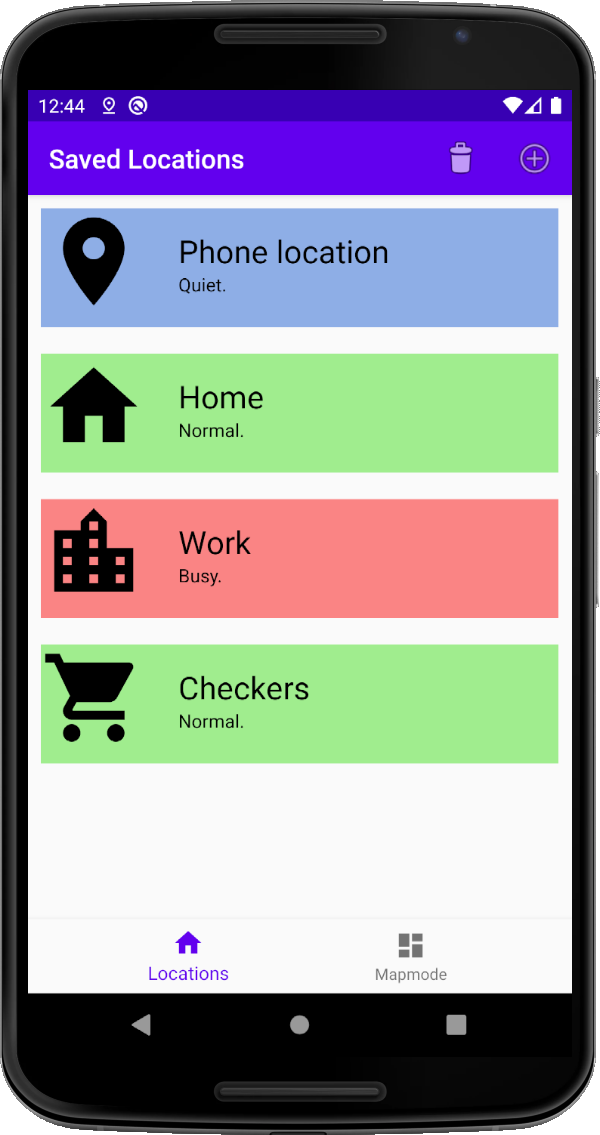
\includegraphics[width=0.268\textwidth]{figures/LocationFragmentDesign.PNG}
    \caption{Location Fragment displaying a user's saved locations with their population status.}
    \label{fig:location_fragment_design}
\end{figure}

Figure \ref{fig:location_fragment_design} is what the app will display once the user has added a number of locations to their saved list. The colour of each location card and status message displayed below each location title will change, depending on the number of people predicted to be at that location currently. The bottom toolbar of this screen allows the user to switch between the two available functions of the Population Density subsystem: the saved-locations fragment and the mapmode fragment. The top toolbar displays the name of the app's view and two interactable buttons. The first of these clears the user's saved locations and the second allows the user to add additional locations. Should the user select this second button, the app will display a fullscreen dialog-fragment. This is an overlay over the current activity which keeps the activity running in the background while the user enters information. This method of input is preferred over creating additional activities or fragments as it simplifies a significant amount of the application layout at the cost of additional processing power. This location input screen is displayed in Figure \ref{fig:enter_location}.

\begin{figure}[ht]
    \centering
    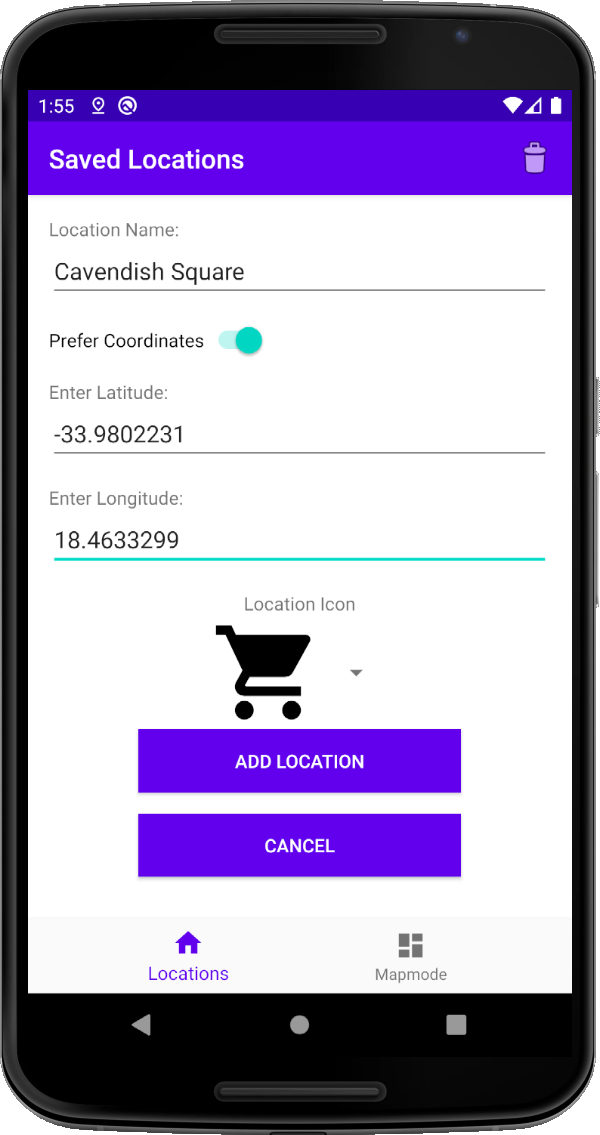
\includegraphics[width=0.268\textwidth]{figures/EnterLocation.PNG}
    \caption{Add-Location View with `prefer coordinates' selected.}
    \label{fig:enter_location}
\end{figure}

The user can use this view to enter both a location's name and coordinates, and then select an appropriate icon to represent the location. A switch is displayed below the name which the user can use to change between entering a location's address or its coordinates. The address functionality is not currently available to the user and acts as a suggestion to future developers of alternative methods of location input. While these figures show the use-case from a consumer's perspective, this functionality can equally apply to business owners, as shown in Figure \ref{fig:business_extended}.

\begin{figure}[ht]
    \centering
    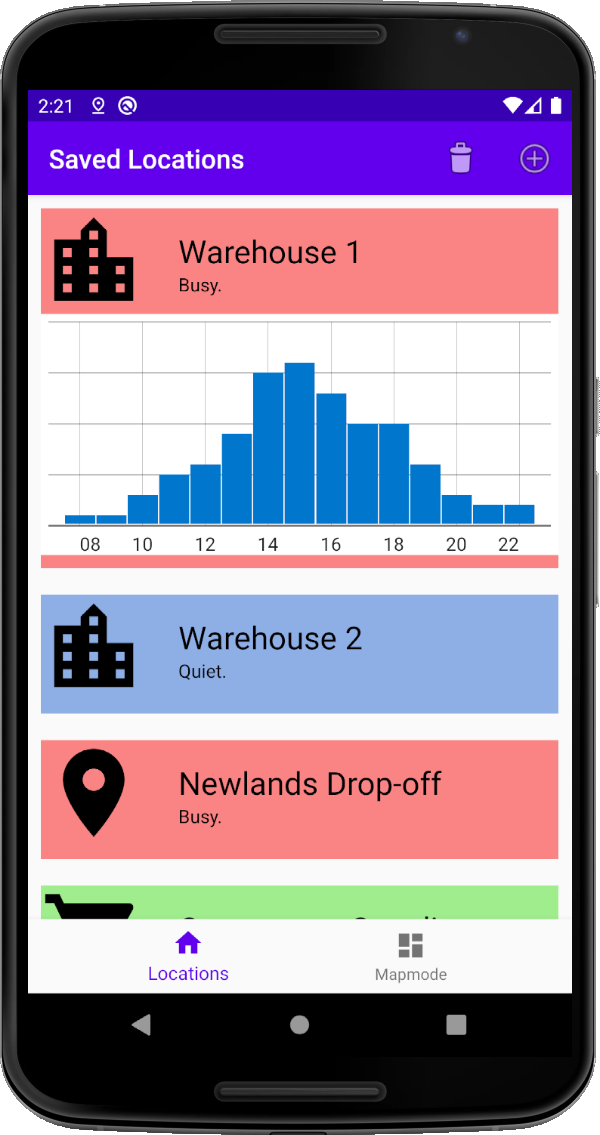
\includegraphics[width=0.268\textwidth]{figures/BusinessExtended.PNG}
    \caption{Location Fragment with a location selected.}
    \label{fig:business_extended}
\end{figure}

Figure \ref{fig:business_extended} is also an example of the Saved-Location Fragment with the first saved-location selected. When such a location is selected, its card will expand to show more detailed information about the predicted population density at that location. In this example, Warehouse 1 is expanded to show what the population is predicted to be throughout the day. Each bar in the graph depicts an hour interval which displays the number of unique users who have previously uploaded their location within 20 meters of the location's coordinates. More detail about how location data is gathered from the server is described in Section \ref{sec:web_interface}.  

Since the time in Figure \ref{fig:business_extended} is 2:21 PM, the app looks at the 14:00-15:00 interval to determine how busy the location is. In this example, this interval is busy compared to the rest of the day, and the app determines this by comparing the current number of people in that time bracket to the maximum difference in population throughout the day. If the number of people is in the top 30\%, it determines the state to be busy, and similarly, the bottom 30\% is determined to be quiet. All other states are displayed as a normal amount of activity. 

\subsubsection{The Mapmode Fragment}

This view is designed as a method of testing the PEEPS framework's ability to perform complex analysis of population data. It initially selects four locations and determines the time one would spend traveling from the first location to each subsequent location at a walking pace. This timestamp and geographical data is then sent to the server which gathers the predicted population density data at those locations. When this data is received back by the app, it will calculate the optimal time that the user could start their journey in order to minimise contact with other individuals.

\begin{figure}[ht]
    \centering
    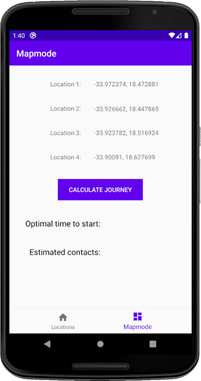
\includegraphics[width=0.268\textwidth]{figures/MapmodeDesign.png}
    \caption{Mapmode Fragment's view displaying four pre-selected locations.}
    \label{fig:mapmode_design}
\end{figure}

When the user selects this view using the bottom toolbar, they will be presented with four predetermined locations and an interactable button. The coordinates of these locations are set up within the app's software and are designed to simulate an environment where the user could input them manually. On selection, the button will start the population calculation and, when completed, the app will present the data near the bottom of the view. The contact prediction functionality is meant to be an example of how population data can be used to provide the user with meaningful information that can be used during the COVID-19 pandemic to minimise contact with potentially infected individuals. This data analysis mechanism could additionally be modified to determine vehicle traffic, population hotspots and the user's likelihood of contracting a seasonal flu.

\section{Server Design and Development}

\subsection{System Description}
The Server system oversees the handling of all user and location requests coming from the application. While this system was designed to be implemented on a local dedicated server, an alternative method that may be more scalable, depending on the network traffic, will be to implement the server using third-party hosting solutions like Amazon EC2 or Google Firebase. These alternative implementations do require outsourcing of server hardware but in turn simplify the development process. For the scope of this project, a local server provides the precise control needed for research testing while still having the capability to store enough data and do so swiftly. 

\subsection{Subsystem Analysis}
The two subsystems that the server utilises are the web interface and database subsystems. These act in tandem so that whenever a request to access database data is sent from the app, the web interface will act as a mediator between the app and the database. For example: if the user wishes to register a new account, the app will collect the user's data into a single JSON variable and forward it to the address of the web interface's \textit{user\_login.php} file. The web interface will then use this data to query the database in order to determine whether there is a conflicting username. Should there be no conflict, the web interface will update the database with the new user's details and return a new JSON variable containing a success message to the application.

\begin{figure}[ht]
    \centering
    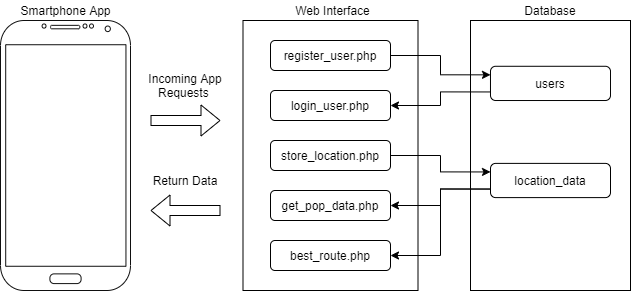
\includegraphics[width=0.85\textwidth]{figures/ServerSubsystemInteraction.png}
    \caption{Server subsystem's interactions with the database and app.}
    \label{fig:server_subsystem_interaction}
\end{figure}

Because the server system was designed to be as modular as possible, each of the web interface programs can interact with the database independently. Similarly, the user interactions and the location-data interactions with the database act as separate functions of the web interface and could even be hosted on different servers if necessary. This open-software development strategy was implemented to ensure that other developers could implement the framework of individual PEEPS systems without having to implement all of the PEEPS functionality.

\subsection{Web Interface Structure}
\label{sec:web_interface}
The web interface of the PEEPS application is hosted using the open source web server solution stack XAMPP. This application was predominantly chosen for its lightweight and cross platform compatibility, making it an appropriate method of web hosting for many situations. While XAMPP allows for a combination of different programming languages, the only one needed for this project is PHP. PHP is a general-purpose scripting language which is predominantly used for web development \cite{ThePHPGroup}. PHP is used in this project for data communication between the local database and the smartphone app and achieves this by manipulating JSON arrays and formatting SQL queries. 

Each PHP application in this subsystem interacts similarly with the PEEPS app. This interaction within the \textit{login\_user.php} program is as follows:

\lstset{style=phpstyle}
\begin{lstlisting}[caption={\detokenize{How login_user.php interacts with the smartphone app.}},label={lst:php_login},language=php]
    <?php
    // Return array as JSON
    $response = array();

    //json data to array
    $content = file_get_contents("php://input");
    $decoded = json_decode($content, true);

    //check for all required fields
    if (isset($decoded['username']) && isset($decoded['password'])) {
    // check if username and password is valid (not shown)
    ... 
    } else {
        // missing field
        $response["success"] = 0;
        $response["message"] = "Required field(s) is missing.";
        //echo response
        echo json_encode($response);
    }
    ?>    
\end{lstlisting}


This figure shows how the program interacts with the smartphone app. When the program starts, it decodes the JSON file and checks whether the correct fields are present. Should these be missing, the program fills a new array with status messages and echos them back to the app once encoded back into JSON format. Should the correct fields be present, the application will instead continue with its database query and return the outcome of the query in addition to the status messages.

\subsubsection{Population Retrieval Algorithm}
Most of the complexity of the web interface is present in the population retrieval programs get\_pop\_data.php and best\_route.php. These programs format complicated SQL queries and return their results as one large dataset. 

\begin{lstlisting}[caption={\detokenize{get_pop_data.php's population-data extraction algorythm. }},label={lst:php_login},language=php]
//connect to DB
$db_con = pg_connect("host=localhost port=5432 dbname=PEEPS user=postgres password=admin");

//assume success until failure
$response["success"] = 1;
$response["message"] = "Data received.";

for ($i=8; $i < 23; $i++) { //for each hour bracket from 8:00 to 23:00
$i2=$i+1; //set end time to be one hour after first
$count = 0;

foreach ($locations as $loc) {

    //format query
    $add_query = "SELECT COUNT(DISTINCT user_id) FROM public.location_data" .
        " WHERE timestamp::date BETWEEN '$previous_date' AND '$current_date'" . 
        // date within 3 weeks
        " AND timestamp::time BETWEEN time '$i:00:00' AND time '$i2:00:00'" . 
        //between hour and hour+1
        " AND EXTRACT(DOW FROM timestamp) = " . $dow . 
        // on day of week of current date
        " AND ST_Distance(ST_Transform('SRID=4326;POINT($loc[0] $loc[1])' ::geometry, 3857), ST_Transform(ST_SetSRID(coordinates,4326),3857))  <= 20"; 
        //within 20 meters of location coordinates

    $result = pg_query($db_con, $add_query);

    //check for errors
    if ($result) {
        //SUCCESS
        $row = pg_fetch_assoc($result);
        // $value = ($row["count"]+0)/$week_scope;
        $response["n".strval($i)."_".strval($i2)."_loc".$count] = $row["count"]+0;

    } else {
        // FAILURE
        $response["success"] = 0;
        $response["message"] = "Data not avaliable.";

        $error = true;
        break;
    }
    $count++;
}
}

//echo response
pg_close();
echo json_encode($response);
}

//echo response
pg_close();
echo json_encode($response);
\end{lstlisting}

This algorythm queries the database for a number of unique users who have have been within 20 meters of the selected location over the last three weeks and also on the current day of the week. It does this for each hour interval between 8 AM and 11 PM and stores this data in an array. Because only the number of users is determined, and not which users, the data is successfully anonymised. When the array is full, it will be converted to JSON format and returned to the app.

\subsection{Database Architecture}
The PostgreSQL database is implemented using the program pgAdmin. This database management tool is both cross-platform and open source, and is currently the most popular platform for developing PostgreSQL databases\cite{pgAdmin}. In addition to the base PostgreSQL installation, the extension PostGIS is utilised to implement location-related objects and functions. This extension is particularly useful for determining distances between locations. This distance is utilised by the web interface to determine the number of datapoints within proximity to a saved location. 

The database consists of two tables: \textit{users} and \textit{location\_data}:

\begin{table}[!htbp]
    \centering
    \begin{tabular}{llll}
    \hline
    \textbf{Field Name} & \textbf{Primary?} & \textbf{Not null?} & \textbf{Type (size)}  \\ \hline
    username   & Yes      & Yes       & VARCHAR (15) \\ \hline
    password   & No       & Yes       & VARCHAR (20) \\ \hline
    \end{tabular}
    \caption{`Users' table field descriptions.}
    \label{tab:des_tab1}
\end{table}



\begin{table}[!htbp]
    \centering
    \begin{tabular}{lllll}
    \hline
    \textbf{Field Name} & \textbf{Primary?} & \textbf{Not null?} & \textbf{Type (size)} & \textbf{Notes}                          \\ \hline
    entry\_id           & Yes               & Yes                & INTEGER              & Autogenerated by database.              \\ \hline
    user\_id            & No                & No                 & VARCHAR (15)         & From `users' table. \\ \hline
    coordinates         & No                & Yes                & GEOMETRY             & Stored in (lon, lat) form.   \\ \hline
    timestamp           & No                & Yes                & TIMESTAMP            & Datatype ignores time zone.             \\ \hline
    \end{tabular}
    \caption{`Location data' table field descriptions.}
    \label{tab:des_tab2}
\end{table}

Table \ref{tab:des_tab2} opts to use the more complicated `geometry' datatype over the simpler `point' type which only stores x/y coordinates. PostGIS's geometry type is built for locational data and can be manipulated to determine distances, geometrical shapes, and areas. While this project mostly uses the distance calculation functionality, the geometry datatype leaves open the possibility for far more complex locational data manipulation.